%%%%%%%%%%%%%%%%%%%%%%%%%%%%%%%%%%%%%%%%%
%
% (c) 2019 by Jennifer Laaser
%
% This work is licensed under the Creative Commons Attribution-NonCommercial-ShareAlike 4.0 International License. To view a copy of this license, visit http://creativecommons.org/licenses/by-nc-sa/4.0/ or send a letter to Creative Commons, PO Box 1866, Mountain View, CA 94042, USA.
%
% The current source for these materials is accessible on Github: https://github.com/jlaaser/pogil-polymers
%
%%%%%%%%%%%%%%%%%%%%%%%%%%%%%%%%%%%%%%%%%

\renewcommand{\figpath}{content/polymphys/solution-thermo/phase-sep/figs}
\renewcommand{\labelbase}{phase-sep}

\begin{activity}{Thermodynamics of Phase Separation}

\begin{instructornotes}

	This activity introduces students to key concepts related to phase diagrams of polymer solutions.
	
	After completing this activity, students will be able to:
			\begin{enumerate}
				\item Explain how the free energy of a polymer solution changes upon phase separation
				\item Articulate the conditions under which a polymer solution will always phase separate, be metastable, or never phase separate
				\item Identify the spinodal and binodal points on a free energy curve
			\end{enumerate}
			
	This activity will prepare students to analyze phase diagrams of polymer solutions in the next activity.
			
	\subsection*{Activity summary:}
	\begin{itemize}
		\item \textbf{Activity type:} Learning Cycle
		\item \textbf{Content goals:} See above %Limits of stability for polymer solutions
		\item \textbf{Process goals:} %https://pogil.org/uploads/attachments/cj54b5yts006cklx4hh758htf-process-skills-official-pogil-list-2015-original.pdf
			\begin{itemize}
				\item Interpreting graphs and equations
				\item Proposing methods for solving a problem
				\item Written and oral communication of reasoning
			\end{itemize}
		\item \textbf{Duration:} Approx. 60 minutes, including class discussion
		
			\emph{Note: for use in a 50-minute class period, students can be asked to work through Model 1 as a warm-up activity prior to class.}
			
		\item \textbf{Instructor preparation required:} none beyond knowledge of relevant content
		\item \textbf{Related textbook chapters:}
			\begin{itemize}
				\item \emph{Polymer Chemistry} (Hiemenz \& Lodge), 2nd ed.: sections 7.5.1-7.5.4
				\item \emph{Introduction to Polymers} (Young \& Lovell), 3rd ed.: not covered in detail
			\end{itemize}
	\end{itemize}

\end{instructornotes}

	%\textbf{Focus question:} Put a central question for the students to consider through this exercise here.

\begin{model}[Free-Energy Curves for Polymer Solutions]

According to Flory-Huggins theory, the free energy of a polymer solution is
\begin{equation*}
	\frac{\Delta G_{mix}^{(int)}}{k_B T} = \phi_1 \phi_2 \chi + \phi_1 \ln \phi_1 + \frac{\phi_2}{N}\ln \phi_2
\end{equation*}
where $\phi_1$ and $\phi_2$ are the volume fractions of solvent and polymer, respectively, $N$ is the degree of polymerization of the polymer, and $\chi$ is the interaction parameter.

This expression is plotted for several different $\chi$ and $N$ values, below:

\centerline{
	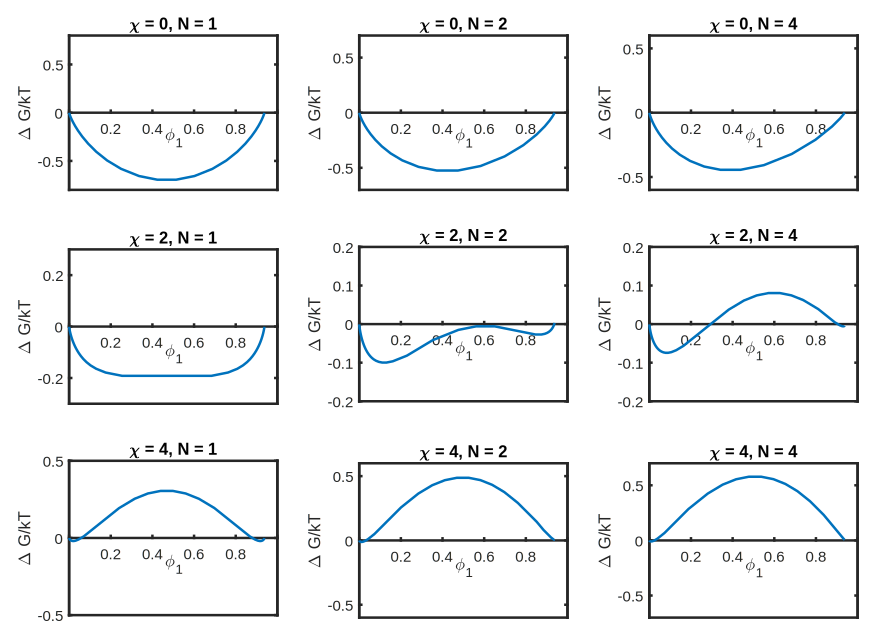
\includegraphics[width=0.9\textwidth]{\figpath/model1_allplots}}

\end{model}

%\vspace{0.05in}
\begin{ctqs}

	\question One of the plots shown in this model corresponds to mixing two identical small-molecule liquids.  Which one is it?  Briefly justify your reasoning.
	
		\begin{solution}[1.5in]
		
			The plot with $\chi=0$ and $N=1$ in the upper left corner corresponds to mixing of two identical small-molecule liquids.
						
			Small-molecule liquids will both have $N=1$, because they are not connected into polymer chains.  Additionally, if they are identical small molecules, then there is no change in the intermolecular interactions on mixing, so $\chi=0$.
			
		\end{solution}
	
	\question Qualitatively, how do the free energy curves change when you...
		\begin{enumerate}
			\item ... increase $\chi$?
	
				\begin{solution}[0.75in]
				
					Increasing $\chi$ causes a ``bump'' to appear in the middle of the curve, causing the curve to have two minima rather than one.  As $\chi$ gets bigger, the minima move further and further toward the edges of the plots.
				
				\end{solution}
				
			\item ... increase $N$?
	
				\begin{solution}[0.75in]
			
					When $N=1$, the curve is perfectly symmetric around $\phi_1=0.5$; increasing $N$ causes the curve to skew to the right.  The depths of the minima are also no longer the same - the one at lower values of $\phi_1$ is deeper.
				
				\end{solution}
		
		\end{enumerate}
		
\end{ctqs}



\begin{model}[Free Energy Changes on Phase Separation]

	When a polymer solution is prepared with a specific volume fraction of solvent $\phi_1$ (which we refer to as a mixture with \emph{composition} $\phi_1$), it can either remain a homogeneous, single-phase mixture with composition $\phi_1$, or it can phase separate into two new phases with different compositions, $\phi_{1A}$ and $\phi_{1B}$, as shown below:
	
		\centerline{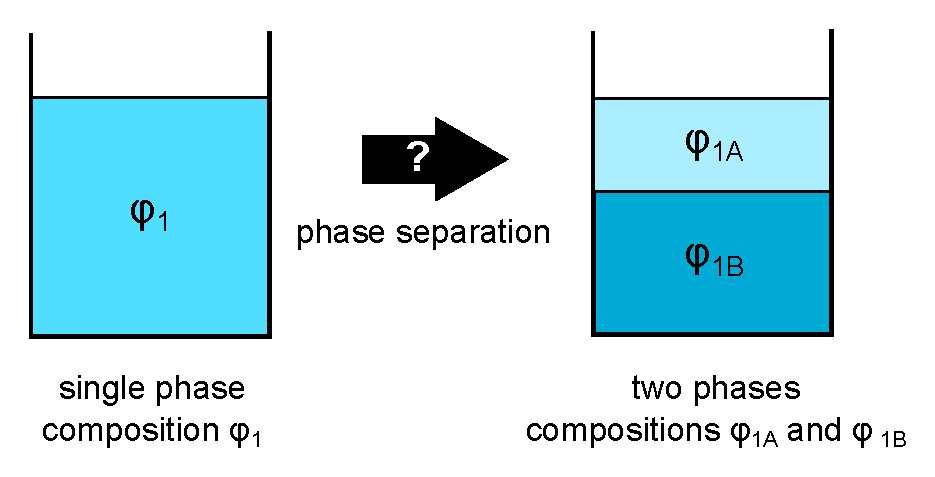
\includegraphics[width=0.6\textwidth]{\figpath/model2-schematic}}
	
	%When this phase separation occurs, the \emph{overall} composition of the sample does not change, but the compositions of the individual phases may be somewhat different from that of the starting mixture.
	
	Working through the math, it turns out that the free energy of the phase-separated mixture falls on a line connecting the free energies of the two individual phases:
	
		\vspace{0.1in}
		\centerline{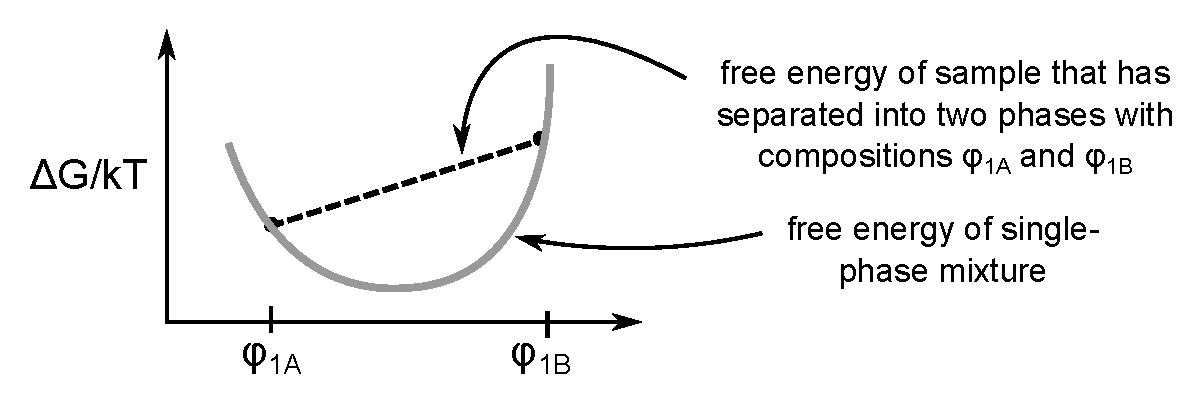
\includegraphics[width=0.75\textwidth]{\figpath/model2-deltaGphasesep}}
	
	If the free energy of the phase-separated mixture is lower than that of the homogeneous solution, the mixture will phase separate; otherwise, it will remain a homogeneous, single-phase solution.

\end{model}

		\vspace{0.1in}
\begin{ctqs}
		\question Consider a section of a free energy curve that is concave down, as shown below:
	
		\vspace{0.1in}
		\centerline{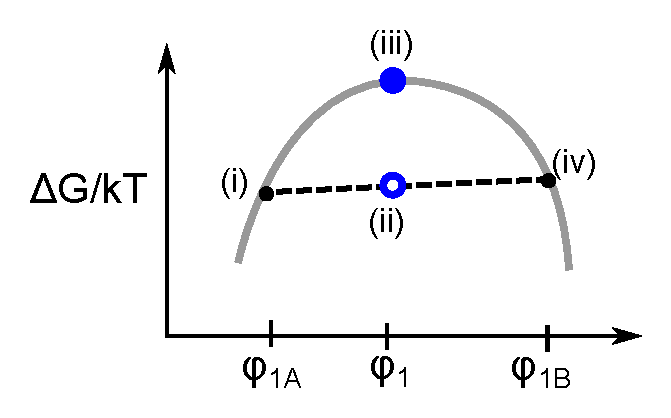
\includegraphics[width=0.5\textwidth]{\figpath/model2-concavedown}}

			\begin{enumerate}
				\item Which point on this plot represents a \emph{homogeneous solution} prepared at composition $\phi_1$?
					
					\begin{solution}[0.75in]
					
						Point (iii) (it is on the curve showing the free energy of a single-phase mixture.)
					
					\end{solution}
					
				\item Which point on this plot represents a mixture with total composition $\phi_1$ that has phase-separated into two phases with compositions $\phi_{1A}$ and $\phi_{1B}$, respectively?
					
					\begin{solution}[0.75in]
					
						Point (ii) (it is on the line connecting the two phase-separated compositions.)
						
					\end{solution}
					
				\item Which state has the lower free energy, the phase-separated state or the homogeneous mixed state?
					
					\begin{solution}[0.75in]
					
						The phase-separated state has a lower free energy.
					
					\end{solution}
					
				\item Would it be favorable for a sample prepared with overall composition $\phi_1$ to separate into two phases with compositions $\phi_{1A}$ and $\phi_{1B}$?  Why or why not?  Briefly explain your answer in 1-2 complete sentences.
					
					\begin{solution}[1.25in]
					
						Yes, it would be favorable for a sample prepared at overall composition $\phi_1$ to phase separate, because the phase-separated state has a lower free energy.
					
					\end{solution}
					
			\end{enumerate}
			
		\clearpage
		\question Next, consider a section of a free energy curve that is concave up, as shown below:
	
		\vspace{0.1in}
		\centerline{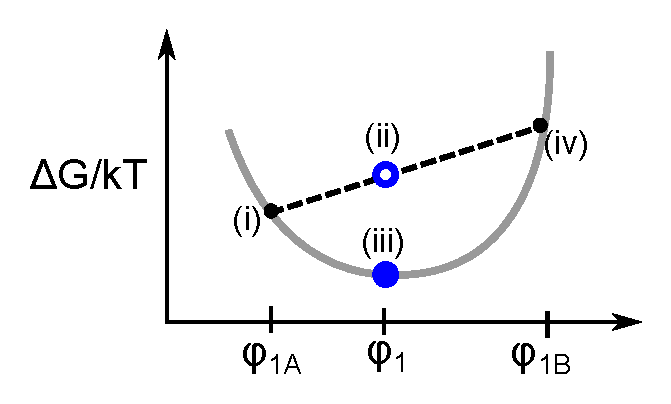
\includegraphics[width=0.5\textwidth]{\figpath/model2-concaveup}}

			\begin{enumerate}
				\item Which point on this plot represents a \emph{homogeneous solution} prepared at composition $\phi_1$?
					
					\begin{solution}[0.75in]
					
						Point (iii) (it is on the curve showing the free energy of a single-phase mixture.)
						
					\end{solution}
					
				\item Which point on this plot represents a mixture with total composition $\phi_1$ that has phase-separated into two phases with compositions $\phi_{1A}$ and $\phi_{1B}$, respectively?
					
					\begin{solution}[0.75in]
					
						Point (ii) (it is on the line connecting the two phase-separated compositions.)
						
					\end{solution}
					
				\item Which state has the lower free energy, the phase-separated state or the homogeneous mixed state?
					
					\begin{solution}[0.75in]
					
						The homogeneous mixed state has a lower free energy.
					
					\end{solution}
					
				\item Would it be favorable for a sample prepared with overall composition $\phi_1$ to separate into two phases with compositions $\phi_{1A}$ and $\phi_{1B}$?  Why or why not?  Briefly explain your answer in 1-2 complete sentences.
					
					\begin{solution}[2in]
					
						No, it would not be favorable for a sample prepared with overall composition $\phi_1$ to phase separate because doing so would raise the free energy of the system.
					
					\end{solution}
					
			\end{enumerate}
			
		\question We can describe these two cases mathematically by looking at the second derivative of $\Delta G$ with respect to $\phi_1$.		
			What is the \emph{sign} of $\frac{\partial^2 \Delta G}{\partial \phi_1^2}$ when...
			
			\begin{enumerate}
				\item ... the free energy curve is concave down?
					
					\begin{solution}[1in]
					
						When the free energy curve is concave down, the second derivative is \emph{negative}.
						
						(Note: some students might find it useful to sketch out a curve and its derivative to arrive at this answer.)
					
					\end{solution}
					
				\item ... the free energy curve is concave up?
					
					\begin{solution}[1in]
					
						When the free energy curve is concave down, the second derivative is \emph{positive}.
						
					\end{solution}
					
			\end{enumerate}
		
		\question Describe, in 2-3 complete sentences, how you could use the second derivative of $\Delta G$ to determine whether or not a mixture prepared at a given composition will phase separate.
					
					\begin{solution}[3in]
					
						To determine whether or not a mixture at a given composition will phase separate, we could first compute the second derivative of the free energy at that composition.  If the second derivative is negative, then it means that the free energy curve is concave down, and the mixture will phase separate.  If, on the other hand, the second derivative is positive, then it means that the free energy curve is concave up, and the mixture will not phase separate.
					
					\end{solution}
					
\end{ctqs}

\clearpage
\begin{model}[Phase Boundaries for Polymer Solutions]
\label{\labelbase:mdl:phaseboundaries}

The free energy curve for a polymer solution with $\chi > 0$ is shown below:

\centerline{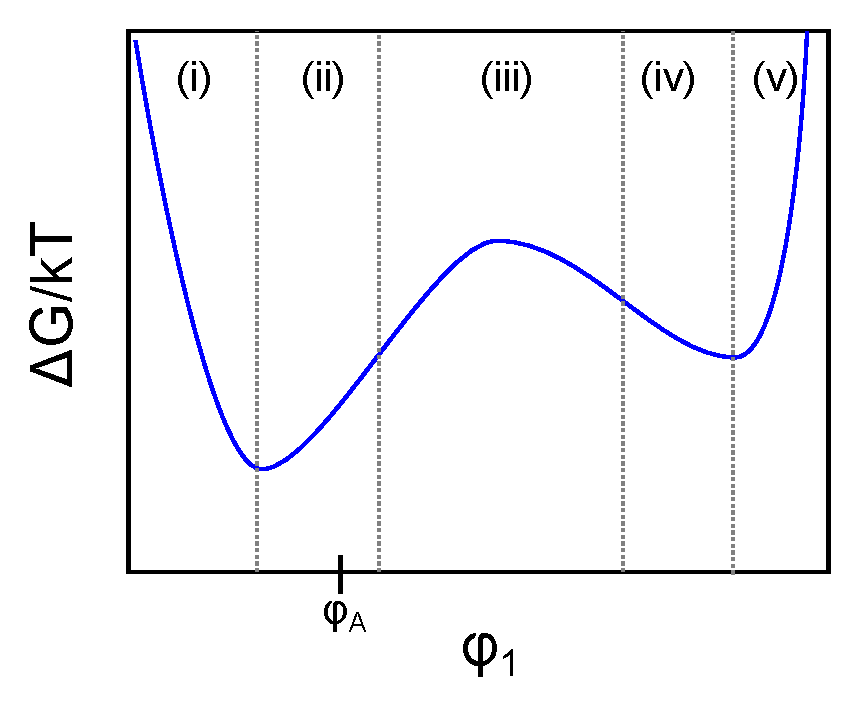
\includegraphics[width=0.5\textwidth]{\figpath/model3-regioncurve}}

\end{model}

\begin{ctqs}

		\question \label{ctq:regionconcavity} In what regions of this plot is the free energy curve...
			\begin{enumerate}
				\item ... concave up?
					
					\begin{solution}[0.75in]
					
						Regions (i), (ii), (iv), and (v)
						
					\end{solution}
				\item ... concave down?
					
					\begin{solution}[0.75in]
					
						Region (iii)
						
					\end{solution}
					
			\end{enumerate}
			
		\question \label{ctq:phaseseplocal} Based \emph{solely} on your answers to CTQ \ref{ctq:regionconcavity}, would you expect a mixture prepared with composition $\phi_1 = \phi_A$ to phase separate?  Briefly explain your reasoning.
					
					\begin{solution}[1.75in]
					
						No. At $\phi_1 = \phi_A$, the free energy curve is concave up, so a mixture prepared at this composition should not phase separate.
					
					\end{solution}
		
		\question \label{ctq:linebelow} Can you draw a line connecting \emph{any} two points on opposite sides of the free energy curve that would pass below the point on the curve at $\phi_1=\phi_A$?  If so, sketch it below:

			\begin{solution}[2.5in]
				\studentdisplay{
					\centerline{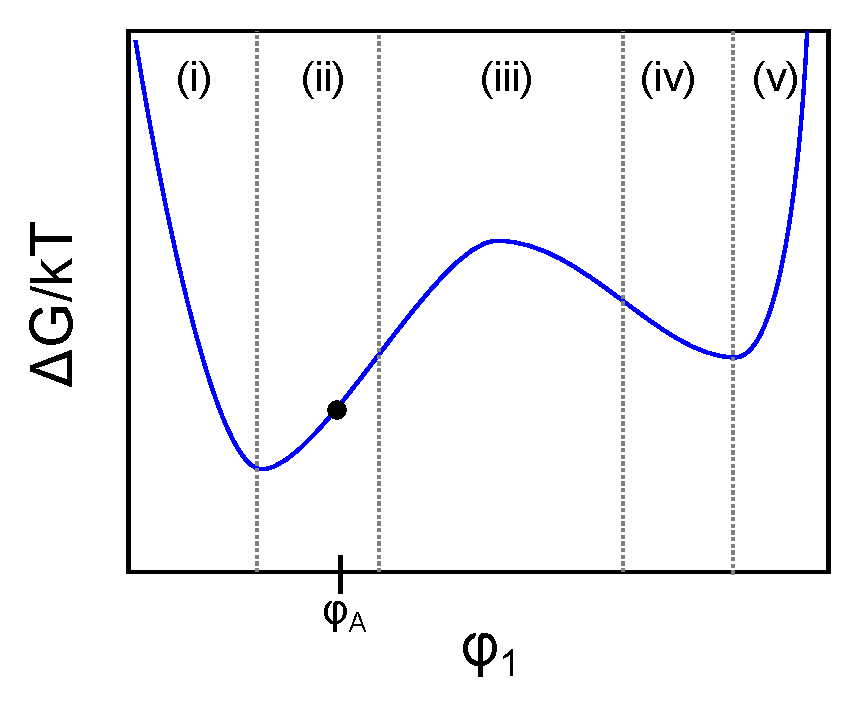
\includegraphics[width=0.55\textwidth]{\figpath/model3-regioncurve-withpt}}
				}
				\instructordisplay{
					\centerline{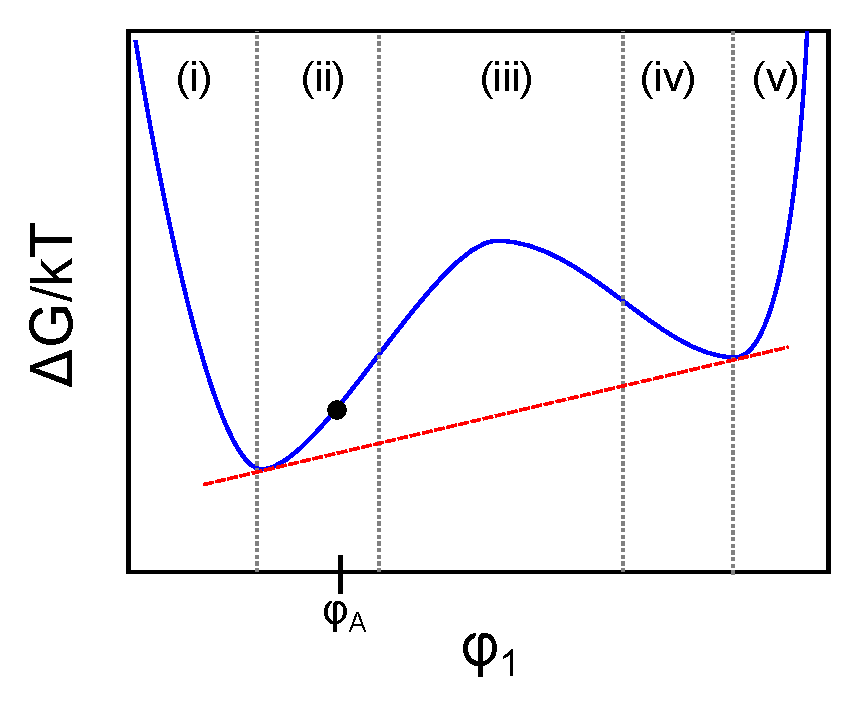
\includegraphics[width=0.35\textwidth]{\figpath/model3-regioncurve-withpt-solution}}
					
					Note: this solution shows the common tangent construction (see solution to question \ref{\labelbase:ctq:findbinodal}), but other lines that pass below the labeled point and intersect the curve on both sides are fine for this question.
				}
			\end{solution}
		
		\question \label{ctq:phasesepglobal} Based \emph{solely} on your answer to CTQ \ref{ctq:linebelow}, would you expect a mixture prepared with composition $\phi_1 = \phi_A$ to phase separate?  Briefly explain your reasoning.
		
			\begin{solution}[1.5in]
			
				Yes.  There is a line connecting two points on the free energy curve that passes below the curve at $\phi_1 = \phi_A$, which means that the free energy of the solution would decrease if it phase-separated into two phases with compositions equal to those where the line connects with the curve.
				
			\end{solution}
		
		\question Do your answers to questions \ref{ctq:phaseseplocal} and \ref{ctq:phasesepglobal} agree?  Why or why not?
		
			\begin{solution}[1.5in]\instructordisplay{
			
				No, they do not agree.  This is because the argument based on the concavity of the curve only works \emph{in the region where the concavity does not change}.  Because the overall free energy curve has some concave down areas, there can still be a phase-separated mixture that decreases the free energy even if the curve is locally concave-up.
				
				Alternatively, students may note that the approach in question \ref{ctq:phaseseplocal} only works when we are considering relatively small changes in composition; it may fail when phase separation results in large changes in the solution composition.
			
			}\end{solution}
			
\end{ctqs}

\begin{infobox}
	In polymer solutions, there are two different ways we can think about phase separation.
	
	First, if there is \emph{any} way to decrease the free energy by undergoing phase separation, then phase separation must be, overall, thermodynamically favorable.
	
	But separating into two phases with very different compositions requires big changes in the local composition, which can be slow, or kinetically unfavorable.
	
	To determine where the \emph{kinetic} limits of phase separation are, we can look at the concavity of the free energy curve:
	\begin{itemize}
		\item If the free energy curve is concave down, then any small fluctuations in local composition will lower the free energy, promoting rapid phase separation.
		\item If the free energy curve is concave up, then any small fluctuations in the local composition will increase the free energy and are unfavorable, hindering phase separation.
	\end{itemize}
	
	Thus, even if it is \emph{thermodynamically} favorable for phase separation to occur, it is possible for it to be \emph{kinetically} unlikely.  We refer to mixtures that are trapped in this sort of local minimum as \emph{metastable}.
	
\end{infobox}

\begin{ctqs}
	\question In which regions of the plot shown in Model \ref{\labelbase:mdl:phaseboundaries} do you expect mixtures to...
		\begin{enumerate}
			\item ... always phase separate?
			
				\begin{solution}[0.5in]
				
					Region (iii)
				
				\end{solution}
			
			\item ... never phase separate?
			
				\begin{solution}[0.5in]
				
					Regions (i) and (v)
				
				\end{solution}
			
			\item ... be metastable?
			
				\begin{solution}[0.5in]
				
					Regions (ii) and (iv)
				
				\end{solution}
				
		\end{enumerate}
		
	\question In 2-3 complete sentences, briefly explain your reasoning for the previous question:
			
				\begin{solution}[2in]
				
					In region (iii), the curve is concave down, so it will always be favorable for the mixture to phase separate.  In regions (ii) and (iv), the curve is concave up, so the mixture will be resistant to small composition fluctuations, but it is possible to draw a line showing that we can lower the free energy if we allow large composition fluctuations, so in these regions the mixture will be metastable.  Finally, in regions (i) and (v), the curve is concave up and it is not possible to draw a line that passes beneath the curve, so in these regions, phase separation is never energetically favorable.
				
				\end{solution}
				
\end{ctqs}

\clearpage
\begin{infobox}
	The points that define the boundaries of the regions that will always spontaneously phase separate are called \emph{spinodal} points.
	
	The points that define the boundaries of the region where phase separation is thermodynamically favorable, even if it might not happen spontaneously, are called \emph{binodal} points.
\end{infobox}

\begin{ctqs}
	\question Locate and label the spinodal points (with an ``S'') and the binodal points (with a ``B'') on the free energy curve shown below:
	
		\begin{solution}[2.5in]
			\studentdisplay{		
				\centerline{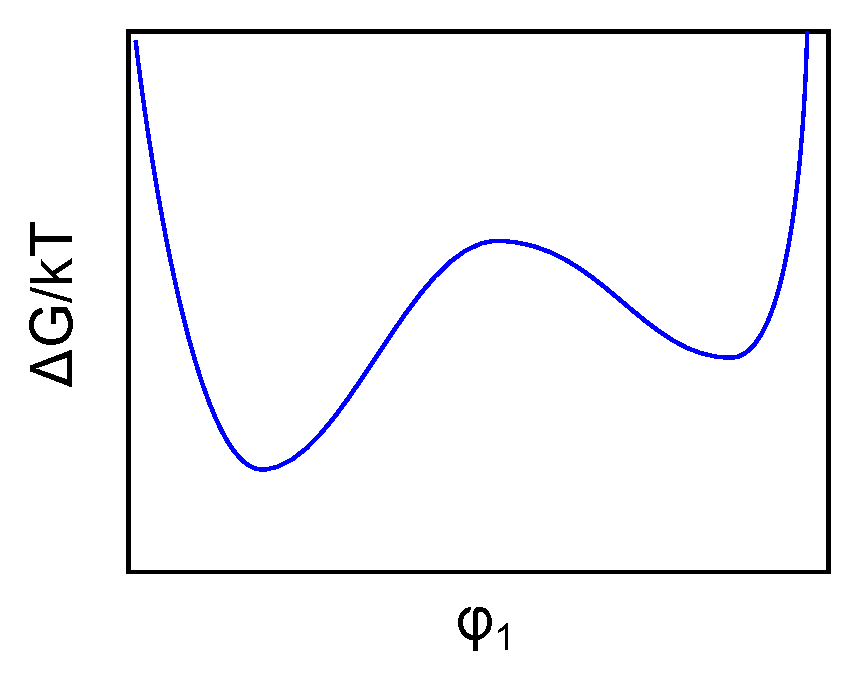
\includegraphics[width=0.5\textwidth]{\figpath/model3-curve}}
			}
			\instructordisplay{	
				\centerline{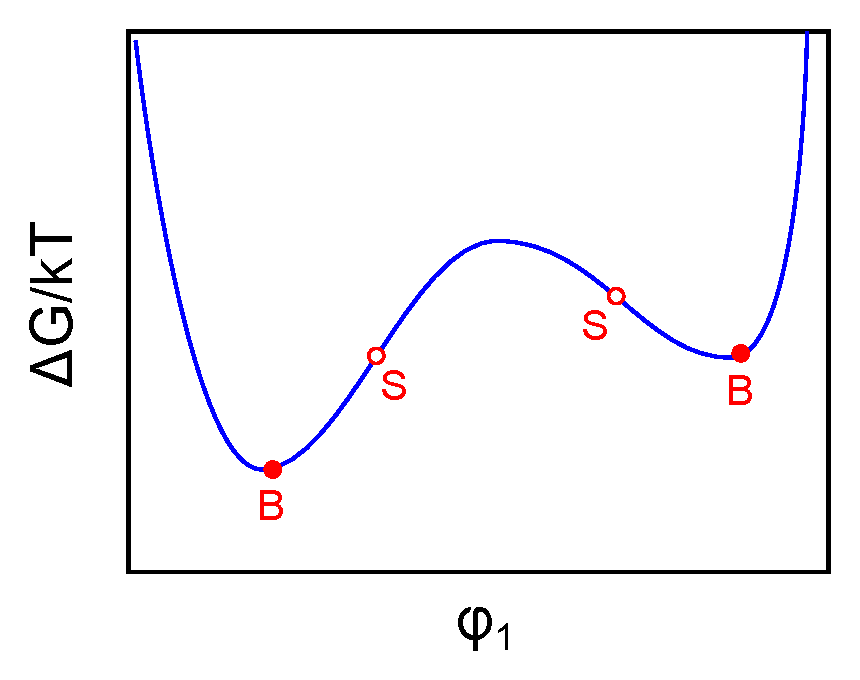
\includegraphics[width=0.5\textwidth]{\figpath/model3-curve-labeled}}
			}
		\end{solution}
	
	\question Propose a \emph{mathematical} method that you could use to find the spinodal points of an arbitrary free energy curve.  Describe your procedure in 2-3 complete sentences.
	
		\emph{Hint: remember that in the concave-up regions, $\frac{\partial^2\Delta G}{\partial \phi_1^2} > 0$ and in the concave-down regions, $\frac{\partial^2\Delta G}{\partial \phi_1^2} < 0$.  What must be true about this derivative at the points where the curve transitions between concave up and concave down?}
		
		\begin{solution}[2.5in]
		
			When the curve transitions from concave up to concave down, the sign of $\frac{\partial^2\Delta G}{\partial \phi_1^2}$ goes from positive to negative.  At the spinodal point, which occurs right at this transition, the value of this derivative must be zero.  Thus, to find the spinodal points, we would just need to find the zeros of $\frac{\partial^2\Delta G}{\partial \phi_1^2}$.
		
		\end{solution}
		
	\question Propose a \emph{graphical} method that you could use to find the binodal points on the free energy curve.  Describe your procedure using 2-3 complete sentences and any diagrams necessary to illustrate your approach.
		\label{\labelbase:ctq:findbinodal}
		
		\begin{solution}[2.5in]\studentdisplay{
		~}\instructordisplay{
		
			Most students will say that they just need to look for the minima in the free energy curve.
			
			This is close, but not quite correct - more precisely, the binodal points are found using the \emph{common tangent construction}, in which we find the line that is \emph{tangent} to both wells in the $\Delta G$ curve; the points where this line touches the $\Delta G$ curve give the binodal compositions.
			
			To illustrate this point, it can be helpful to sketch the following curve for students:
			
\centerline{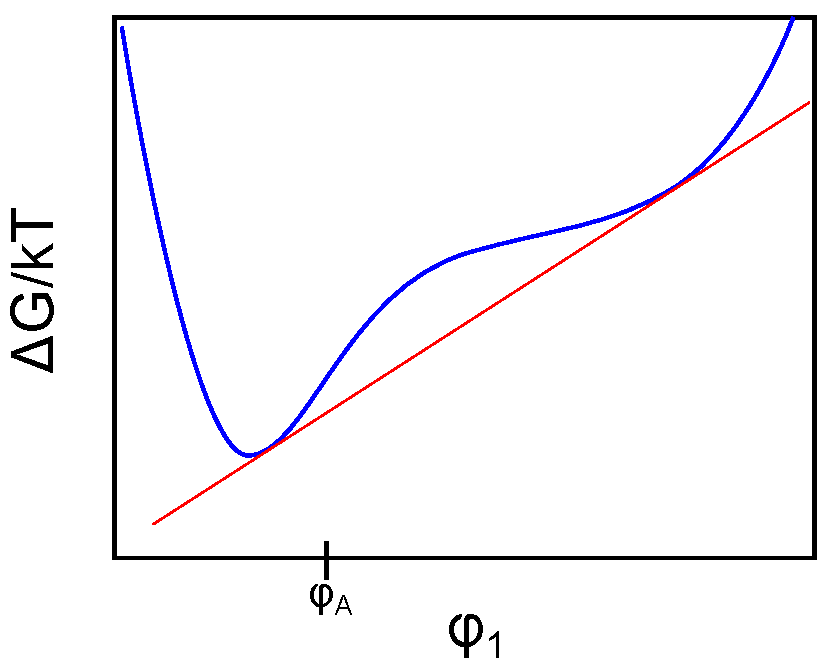
\includegraphics[width=0.3\textwidth]{\figpath/model3-notwominima}}			
			
			This curve only has one local minimum, on the left side, but sketching the common tangent clearly indicates that there is a second binodal point on the right-hand side of the plot.
		
		
		}\end{solution}
		
\end{ctqs}



\begin{exercises}
		
		\exercise Find the spinodal points for a polymer solution whose free energy is given by
		
			\begin{equation*}
				\frac{\Delta G_{mix}^{(int)}}{k_B T} = \phi_1\phi_2\chi + \phi_1\ln\phi_1 + \frac{\phi_2}{N}\ln\phi_2
			\end{equation*}
			
			You will find it helpful to remember that $\phi_2 = 1-\phi_1$.
		
			\begin{solution}\instructordisplay{
				First, rewrite the free energy in terms of only $\phi_1$:
				\begin{equation*}
					\frac{\Delta G_{mix}^{(int)}}{k_B T} = \phi_1(1-\phi_1)\chi + \phi_1\ln\phi_1 + \frac{(1-\phi_1)}{N}\ln(1-\phi_1)
				\end{equation*}
			
				Next, calculate the first and second derivatives:
				\begin{align*}
					\frac{d\Delta G}{d\phi_1} &= \chi\left(\phi_1(-1) + 1(1-\phi_1)\right) + \left(1\ln\phi_1 + \phi_1\frac{1}{\phi_1}\right) + \frac{1}{N}\left((-1)\ln(1-\phi_1) + (1-\phi_1)\frac{-1}{1-\phi_1}\right)\\
						&= \chi\left(1-2\phi_1\right) + \left(\ln\phi_1 + 1\right) - \frac{1}{N}\left(\ln(1-\phi_1) + 1\right)\\
				\end{align*}
				}\end{solution}% break is needed to fix page break issues
				\begin{solution}\instructordisplay{
				and
				\begin{align*}
					\frac{d^2\Delta G}{d\phi_1^2} &= \frac{d}{d\phi_1}\frac{d\Delta G}{d\phi_1}\\
						&= \frac{d}{d\phi_1}\left[\chi\left(1-2\phi_1\right) + \left(\ln\phi_1 + 1\right) - \frac{1}{N}\left(\ln(1-\phi_1) + 1\right)\right]\\
						&= \chi(0 - 2) + \left(\frac{1}{\phi_1} + 0\right) - \frac{1}{N}\left(\frac{-1}{1-\phi_1} + 0\right)\\
						&= -2\chi + \frac{1}{\phi_1} + \frac{1}{N}\frac{1}{1-\phi_1}
				\end{align*}
				
				This second derivative is equal to zero when
				\begin{align*}
					-2\chi + \frac{1}{\phi_1} + \frac{1}{N}\frac{1}{1-\phi_1} &= 0\\
					\frac{1}{\phi_1} + \frac{1}{N}\frac{1}{1-\phi_1} &= 2\chi \\
					1-\phi_1 + \frac{\phi_1}{N} &= 2\chi\phi_1(1-\phi_1) \\
					1-\phi_1 + \frac{\phi_1}{N} &= 2\chi\phi_1-2\chi\phi_1^2 \\
					2\chi\phi_1^2 - \left(\frac{1}{N} - 1 - 2\chi\right)\phi_1 + 1 &= 0
				\end{align*}
				which, using the quadratic formula, yields
				\begin{align*}
					\phi_1 &= \frac{\left(\frac{1}{N} - 1 - 2\chi\right) \pm \sqrt{\left(\frac{1}{N} - 1 - 2\chi\right)^2 - 4(2\chi)(1)}}{2(2\chi)}
				\end{align*}
			}\end{solution}
\end{exercises}
	
\end{activity}